\documentclass[12pt]{article}

\usepackage{amssymb}
\usepackage{multicol}
\usepackage[top=5em, bottom=5em, left=5em, right=5em]{geometry}
\usepackage{listings}
\usepackage{tikz}
\usetikzlibrary{positioning}

\setlength\parindent{0em}
\setlength\parskip{1em}

\title {Assignment 5}

\author {Hendrik Werner s4549775}

\begin{document}
\maketitle

This was done in collaboration with Constantin Blach (s4329872).

\section{} %1
\section{} %2
We worked out the following algorithm:

\begin{lstlisting}
A <- bellman_ford(G)
ratings <- []

for u, v in E'
	G' <- (A.V, union(A.E, (u, v)))
	for u', v' in {(u', v') in G'.E | reachable(u, u')}
		relax(u', v')
	append(ratings, t)

sort(E', ratings)
output "Build road %s", head(E')
\end{lstlisting}

Where $G$ is the given graph, $E'$ the set of proposed roads, $A.E$ is the set of edges of graph $A$, $A.V$ is the set of vertices for graph $A$, $relax(e)$ relaxes edge $e$, $sort(A, b)$ sorts $A$ by $b$ (in increasing order), $head(L)$ returns the first element from list $L$, $reachable(a, b)$ return whether $b$ can be reached from $a$, and $union(A, B) = A \cup B$.

\section{} %3
\textbf{Note: On the exercise sheet there is a contradiction:} it says to use $z$ as a starting node but in the picture just below that it shows $s$ to be the starting node. As I did not know which one was correct and because $s$ is a conventional name for the starting node I chose for $s$ as the starting point.

My partner Constantin Blach chose for $z$ as the starting point and we performed the algortihm on both but each only wrote one down. You can see the other version on the sheet he handed in.

Initial state:

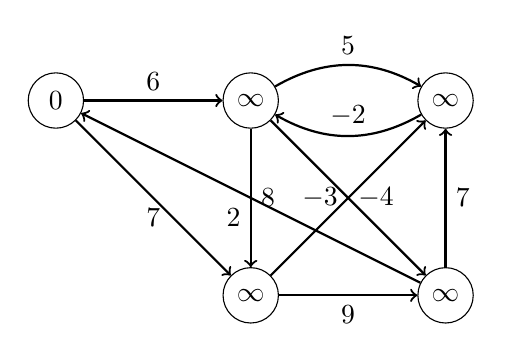
\begin{tikzpicture}[baseline=(s.north), node distance=5em, c/.style={circle, draw, minimum width=2em}]
	\node[c] (s) {$0$};
	\node[c, right=of s] (t) {$\infty$};
	\node[c, right=of t] (x) {$\infty$};
	\node[c, below=of t] (y) {$\infty$};
	\node[c, below=of x] (z) {$\infty$};

	\path[->, thick] (s) edge node [auto] {$6$} (t);
	\path[->, thick] (s) edge node [below] {$7$} (y);
	\path[->, thick, bend left] (t) edge node [auto] {$5$} (x);
	\path[->, thick] (t) edge node [auto] {$8$} (y);
	\path[->, thick] (t) edge node [right] {$-4$} (z);
	\path[->, thick, bend left] (x) edge node [above] {$-2$} (t);
	\path[->, thick] (y) edge node [left] {$-3$} (x);
	\path[->, thick] (y) edge node [below] {$9$} (z);
	\path[->, thick] (z) edge node [auto] {$2$} (s);
	\path[->, thick] (z) edge node [right] {$7$} (x);
\end{tikzpicture}

$|V| = 5$ so we need to do $5 - 1 = 4$ iterations.

$(u, v) \rightarrow x$ denotes that after the relaxation of edge $(u, v)$ vertex $x$ has a weight of $x$.

\begin{enumerate}
	\item
	Relaxation:
	\begin{multicols}{3}
		\begin{description}
			\item[$(t, x)$] $\rightarrow \infty$
			\item[$(t, y)$] $\rightarrow \infty$
			\item[$(t, z)$] $\rightarrow \infty$
			\item[$(x, t)$] $\rightarrow \infty$
			\item[$(y, x)$] $\rightarrow \infty$
			\item[$(y, z)$] $\rightarrow \infty$
			\item[$(z, x)$] $\rightarrow \infty$
			\item[$(z, s)$] $\rightarrow 0$
			\item[$(s, t)$] $\rightarrow 6$
			\item[$(s, y)$] $\rightarrow 7$
		\end{description}
	\end{multicols}

	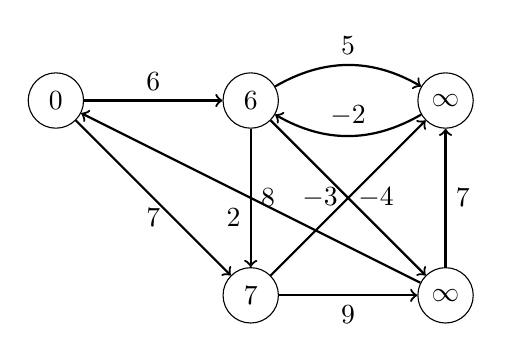
\begin{tikzpicture}[baseline=(s.north), node distance=5em, c/.style={circle, draw, minimum width=2em}]
		\node[c] (s) {$0$};
		\node[c, right=of s] (t) {$6$};
		\node[c, right=of t] (x) {$\infty$};
		\node[c, below=of t] (y) {$7$};
		\node[c, below=of x] (z) {$\infty$};

		\path[->, thick] (s) edge node [auto] {$6$} (t);
		\path[->, thick] (s) edge node [below] {$7$} (y);
		\path[->, thick, bend left] (t) edge node [auto] {$5$} (x);
		\path[->, thick] (t) edge node [auto] {$8$} (y);
		\path[->, thick] (t) edge node [right] {$-4$} (z);
		\path[->, thick, bend left] (x) edge node [above] {$-2$} (t);
		\path[->, thick] (y) edge node [left] {$-3$} (x);
		\path[->, thick] (y) edge node [below] {$9$} (z);
		\path[->, thick] (z) edge node [auto] {$2$} (s);
		\path[->, thick] (z) edge node [right] {$7$} (x);
	\end{tikzpicture}

	\item
	Relaxation:
	\begin{multicols}{3}
		\begin{description}
			\item[$(t, x)$] $\rightarrow 11$
			\item[$(t, y)$] $\rightarrow 7$
			\item[$(t, z)$] $\rightarrow 2$
			\item[$(x, t)$] $\rightarrow 6$
			\item[$(y, x)$] $\rightarrow 4$
			\item[$(y, z)$] $\rightarrow 2$
			\item[$(z, x)$] $\rightarrow 4$
			\item[$(z, s)$] $\rightarrow 0$
			\item[$(s, t)$] $\rightarrow 6$
			\item[$(s, y)$] $\rightarrow 7$
		\end{description}
	\end{multicols}

	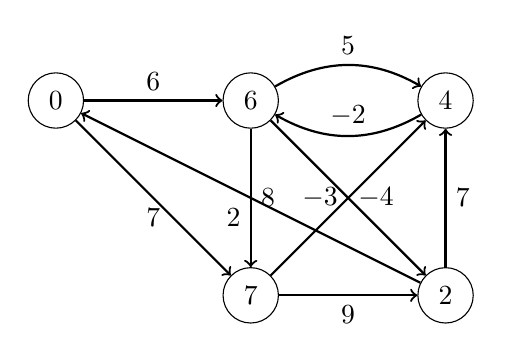
\begin{tikzpicture}[baseline=(s.north), node distance=5em, c/.style={circle, draw, minimum width=2em}]
		\node[c] (s) {$0$};
		\node[c, right=of s] (t) {$6$};
		\node[c, right=of t] (x) {$4$};
		\node[c, below=of t] (y) {$7$};
		\node[c, below=of x] (z) {$2$};

		\path[->, thick] (s) edge node [auto] {$6$} (t);
		\path[->, thick] (s) edge node [below] {$7$} (y);
		\path[->, thick, bend left] (t) edge node [auto] {$5$} (x);
		\path[->, thick] (t) edge node [auto] {$8$} (y);
		\path[->, thick] (t) edge node [right] {$-4$} (z);
		\path[->, thick, bend left] (x) edge node [above] {$-2$} (t);
		\path[->, thick] (y) edge node [left] {$-3$} (x);
		\path[->, thick] (y) edge node [below] {$9$} (z);
		\path[->, thick] (z) edge node [auto] {$2$} (s);
		\path[->, thick] (z) edge node [right] {$7$} (x);
	\end{tikzpicture}

	\item
	Relaxation:
	\begin{multicols}{3}
		\begin{description}
			\item[$(t, x)$] $\rightarrow 4$
			\item[$(t, y)$] $\rightarrow 7$
			\item[$(t, z)$] $\rightarrow 2$
			\item[$(x, t)$] $\rightarrow 2$
			\item[$(y, x)$] $\rightarrow 4$
			\item[$(y, z)$] $\rightarrow 2$
			\item[$(z, x)$] $\rightarrow 4$
			\item[$(z, s)$] $\rightarrow 0$
			\item[$(s, t)$] $\rightarrow 2$
			\item[$(s, y)$] $\rightarrow 7$
		\end{description}
	\end{multicols}

	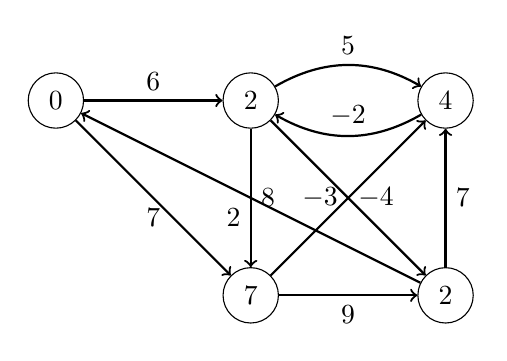
\begin{tikzpicture}[baseline=(s.north), node distance=5em, c/.style={circle, draw, minimum width=2em}]
		\node[c] (s) {$0$};
		\node[c, right=of s] (t) {$2$};
		\node[c, right=of t] (x) {$4$};
		\node[c, below=of t] (y) {$7$};
		\node[c, below=of x] (z) {$2$};

		\path[->, thick] (s) edge node [auto] {$6$} (t);
		\path[->, thick] (s) edge node [below] {$7$} (y);
		\path[->, thick, bend left] (t) edge node [auto] {$5$} (x);
		\path[->, thick] (t) edge node [auto] {$8$} (y);
		\path[->, thick] (t) edge node [right] {$-4$} (z);
		\path[->, thick, bend left] (x) edge node [above] {$-2$} (t);
		\path[->, thick] (y) edge node [left] {$-3$} (x);
		\path[->, thick] (y) edge node [below] {$9$} (z);
		\path[->, thick] (z) edge node [auto] {$2$} (s);
		\path[->, thick] (z) edge node [right] {$7$} (x);
	\end{tikzpicture}

	\item
	Relaxation:
	\begin{multicols}{3}
		\begin{description}
			\item[$(t, x)$] $\rightarrow 4$
			\item[$(t, y)$] $\rightarrow 7$
			\item[$(t, z)$] $\rightarrow -2$
			\item[$(x, t)$] $\rightarrow 2$
			\item[$(y, x)$] $\rightarrow 4$
			\item[$(y, z)$] $\rightarrow -2$
			\item[$(z, x)$] $\rightarrow 4$
			\item[$(z, s)$] $\rightarrow 0$
			\item[$(s, t)$] $\rightarrow 2$
			\item[$(s, y)$] $\rightarrow 7$
		\end{description}
	\end{multicols}

	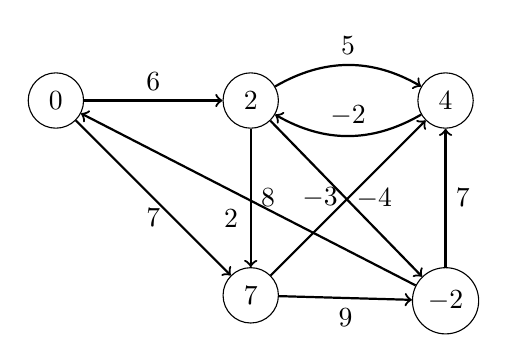
\begin{tikzpicture}[baseline=(s.north), node distance=5em, c/.style={circle, draw, minimum width=2em}]
		\node[c] (s) {$0$};
		\node[c, right=of s] (t) {$2$};
		\node[c, right=of t] (x) {$4$};
		\node[c, below=of t] (y) {$7$};
		\node[c, below=of x] (z) {$-2$};

		\path[->, thick] (s) edge node [auto] {$6$} (t);
		\path[->, thick] (s) edge node [below] {$7$} (y);
		\path[->, thick, bend left] (t) edge node [auto] {$5$} (x);
		\path[->, thick] (t) edge node [auto] {$8$} (y);
		\path[->, thick] (t) edge node [right] {$-4$} (z);
		\path[->, thick, bend left] (x) edge node [above] {$-2$} (t);
		\path[->, thick] (y) edge node [left] {$-3$} (x);
		\path[->, thick] (y) edge node [below] {$9$} (z);
		\path[->, thick] (z) edge node [auto] {$2$} (s);
		\path[->, thick] (z) edge node [right] {$7$} (x);
	\end{tikzpicture}
\end{enumerate}

After another round of relaxation nothing changes so there are no negatively weighted circles.

\section{} %4
We can treat the currencies $c_1, c_2, \dots, c_n$ as vertices and the exchange rates $r_{i, j}$ as directed edges $(c_i, c_j)$ with weight $r_{i, j}$. $G = (V, E), V = c_1, c_2, \dots, c_n, E = \{r_{i, j}\ |\ i, j \in \mathbb{N^+}, i \leq n, j \leq n\}$

We want to find the optimal path from $s \in V$ to $t \in V$. The optimal path is defined as the path that maximises the output of $t$. This is the path with the highest accumulative exchange rate. There may not exists an optimal path if $G$ contains circles with an accumulative exchange rate greater than $1$.

Exchange rates are accumulated by multiplication.

We can find the optimal path by modifying the Bellman-Ford algorithm:

\begin{lstlisting}
d[s] <- 0
for v in V - s
	d[v] <- infinity

for i in 1..|V|-1
	for u, v in E
		if d[v] < d[u] * w(u, v)
			d[v] <- d[u] * w(u, v)

for u, v in E
	if d[v] < d[u] * w(u, v)
		throw MoneyPrintingMachineException
\end{lstlisting}

Where $infinity = \infty$ and $w(u, v) = r_{u, v}$ and $MoneyPrintingMachineException$ indicates that we found a loop with an accumulative exchange rate greater than $1$ which means we can make money by taking this loop so there is no optimal path as we can always increase the accumulative exchange rate by taking another round trip in this loop.

\section{} %5

\end{document}
